\begin{comment}
	- Comparación c y asm.
		- La mayor diferencia es que se levanta de a más.
	- El tiempo en asm es súper constante porque sólo depende de size. En c mas o menos, explicar por qué.
	- Hay un caso límite. Explicar. Aunque se trata como un chorizo.
	- Explicar optimización del acceso a memoria.
	- Explicar por qué no se puede hacer tanta ejcución fuera de orden. Hay dependencia de datos.
	- ¿Que pesa más?¿Procesamiento o acceso a memoria?

\end{comment}

\subsection{Descripción del filtro}

	El filtro consite en extraer un mensaje codificado detro de la imagen conociendo
, por supuesto la menera en que este está codificado.

	La codificación consiste en cambiar cambiar en cada byte de la imagen los
dos bits menos significativos por los bits del mensaje. Es decir que cada
byte del mensaje de codifica en 4 bytes de la imagen (2 bits en cada imagen).

	Es decir que la imagen está alterada, pero está los cambios son tan leves
que no son visibles al ojo humano. Es mucho mayor la variación de colores que
se produce por ver la imagen en diferentes monitores que la que se produce
por cambiar estos bits.

	Los pares de bits, además tienen una breve codificación individual. Que
se determina mirando los bits 2 y 3 de cada Byte. Es decir que uno sabe
como interpretar los dos bits menos significativos mirando los siguientes
2 bits.


\subsection{Implementaciones}


	Para decode se usaron 3 implementaciones: Una escrita en lenguaje C.
Una escrita en lenguaje ensamblador y otra escrita en lenguaje ensamblador
intentando usar la máximo los beneficios de la ténica de software pipelining.

	El algorítmo de C al igual que en los otros filtros es lo mas intuitivo posible.
Basicamente se lee de a un byte de la imagen. Mediante máscaras se filtran los dos bits
menos significativos y los siguientes 2 bits menos significativos.

	Los bits 2 y 3 se comparan en un switch para saber como procesar
a los bits 0 y 1. Una vez que se procesaron los bits 0 y 1 se los guarda se los
mueve a izquierda la cantida de lugares adecuada (0, 2, 4 o 6) según sea el primer
par de bits de ese bytes, el segundo, el tercero o el cuarto. Luego se van acumulando
esos resultados parciales y cuando se tiene un byte entero se lo guarda en el vector
destino.

	Cabe aclarar que a la hora de implementar en ensamblador este filtro provee bastantes
facilidades. Todos los corrimientos que hay que hacer son múltiplos de dos y la cantidad
de datos que hacen falta decodidificar para formar un byte es potencia de 2. Estas
cosas facilitaron mucho el trabajo. Además en ningún momento se necesita saber la
posición de los pixeles ni nada por el estilo, por lo que la matriz fuente se puede
tomar sencillamente como un gran vector.

	El proceso, entonces, es sencillo:

\begin{enumerate}

	\item Se traen datos de la matriz fuente a un registro xmm. Una vez que
	están en registro estos datos se copian a otro xmm

	\item En una de las copias se conservan los bits 0 y 1. En otra los bits 0 y 3.

	\item A todos los bits se los hace pasar por el proceso de sumar, restar
	y negar. Sin embargo lo que se hace es usar una máscara para poner diferentes operandos
	en cada uno. Por ejemplo cuando se realiza la suma sólo aquellos valores
	a los que corresponde sumar tienen como segundo operando un uno, el resto tiene
	un cero. Para que esto quede así se repiten los siguientes pasos para cada
	posicle operación:

	\begin{enumerate}

		\item Se compara el registro que tiene los bits 2 y 3 con una
		máscara que contiene la referencia a la operación a realizar repetida
		en cada byte. Por ejemplo la máscara de negar tiene 0x0C en todos sus bytes.

		\item Cada vez que se compara con una máscara luego se realiza una conjunción
		con otra máscara que tiene el segundo operando de la operación a relizar.
		Por ejemplo si lo que hay que hacer es la dato sumarle uno entonces
		Se usa una máscara de unos. En el resto de las posiciones queda cero.

		\item Por último se realiza la operación entre los datos (es decir los bits
		menos significativos de los bytes traídos de la imagen) y la máscara recién
		creada.

	\end{enumerate}

	\item Una vez realizado 4 cuartetos de pares de bits alineados. Para que ocupen las
	posiciones adecuadas, entonces, lo qeu se hace es realizar 4 copias, shiftear de
	manera empaquetada , 0 , 2 , 4 y 6 lugares respectivamente y por último sumar todo.
	
	\item Ahora se tienen 4 bytes armados pero desordenados. Es necesario tenerlos todos
	en la parte baja del registro para poder grabar a memoria. Esto se hace mediante un shuffle
	de bytes.

	\item Al final del ciclo existe un caso complicado. El tamaño del string de salida
	no tiene por qué ser múltiplo de 4 (hasta ahora se estuvieron insertando de a 4
	bytes a la vez). Para resolver esto se implementó una lógica especial
	intentando que reste la menor cantidad de performance posible. Sólo se entra al código
	que describe esta lógica en la anteúltima y en la última iteración.

\end{enumerate}


\subsection{Optimizaciones}

	Se intentó utilizar el entubado de código ($software pipelining$) de diversas maneras.
En un principio se dividió el proceso en 4 etapas: Acceso a memoria por un lado
y por otro los 3 entradas del switch. Sin embargo esto no produjo mejoras en la performance,
por el contrario disminuyó. Por lo tanto se bajó un poco el nivel de ambición y se realizaron
sólo 2 etapas. Por un lado el acceso a memoria y por el otro lado el proceso de los datos. La idea
era lograr que el proceso siga mientras se realiza el acceso a memoria en lugar de tener que esperar.
El proceso fue el siguiente:

	Antes de entrar al ciclo se traen los datos necesarios para hacer la priemra iteración.
Una vez adentro del ciclo se traen los datos necesarios para la segunda iteración, pero
se trabaja con los datos que ya se trajeron antes. Luego al finalizar el ciclo.
Se mueven los datos traídos al principio del ciclo al registro en el cuál se trabaja.

	El resultado de esto es que las operaciones no tienen dependencias a nivel de datos con
la lectura de memoria, por lo tanto el procesador no tienen que esperar a que se termine el ciclo
de lectura para poder empezar a trabajar con los datos.

	A nivel de código la optimización es súper sencilla. Mucho mucho más que la enterior.
Bastó con agregar unas pocas líneas de código en el lugar adecuado para aumentar en un 15\% la performance
con respecto al código original. Un par de pruebas nos mostraron que el lugar óptimo para hacer el último
movimiento es lo mas cerca del final del ciclo posible.

\subsection{Rendimiento}

\begin{figure}[h]
\begin{center}
  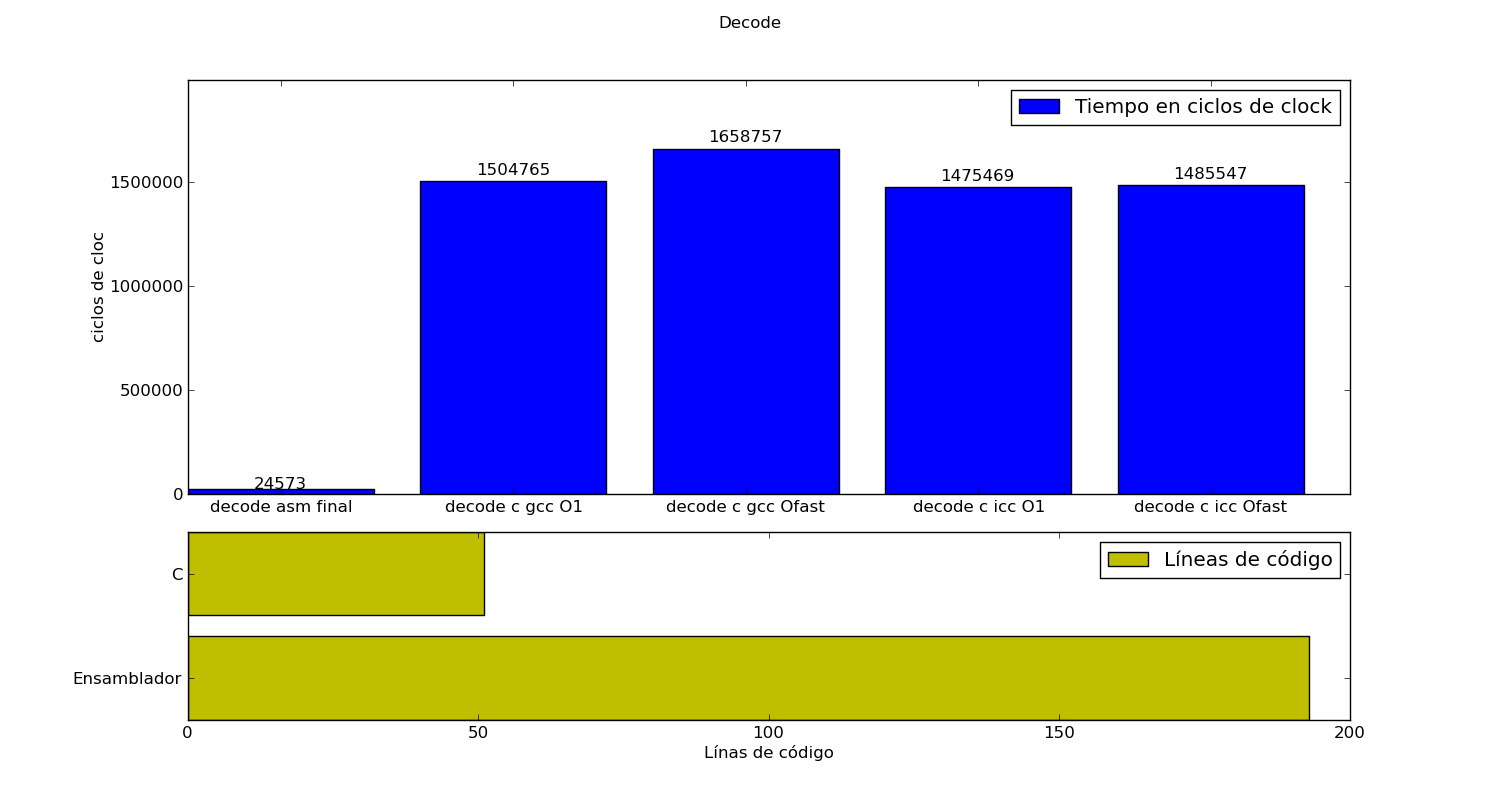
\includegraphics[scale=0.4]{secciones/decodificacion/imagenes/decode.png}
\end{center}
\caption{Imagen antes y después de aplicar el filtro de color con color principal rojo.}
\label{fig:filtro-color-ejemplo}
\end{figure}

	Como se puede ver en el gráfico el rendimiento de la versión en assembler es notablemente mas rápida. Otra
vez no cumple con la hipótesis inicial. La versión en ASM es más de 60 veces mas rápida que la versión
de C. Al introducir ICC en la ecuación la cosa cambia un poco, sin embargo el resultado sigue siendo que
la versión en ensamblador aplasta a las demás.

	En este momento cabe volver a mencionar que este filtro calza a la perfección en el procesamiento
SIMD con SSE. Aclarado esto vamos a ahondar un poco más.

	La versión de C siguiendo el código tal cuál está escrito accede a memoria 5 veces cada 4 bytes.
Es decir, tiene que buscar cada byte. Luego de procesar 4 bytes tiene que ir a guardarlos. Es decir
que suponiendo que el compilador genera un código que no accede nunca a memoria durante el ciclo de todas
maneras se están accediendo 20 veces a memoria cada 16 bytes. La versión escita en ensamblador, en cambio
realiza sólo 2 accesos cada 16 bytes (uno para traer datos, otro para guardarlos). Pero no sólo eso sino
que además el acceso mas conflictivo (el de trar datos) está optimizado mediante entubado de código.

	Otra cosa importante a la hora de hacer este análisis es que se sabe con mucha presición
cuantas veces se realiza el ciclo principal. Si o si está en el orden de $size/4$ veces. Es decir,
en cada iteración se graban exactamente 4 bytes y las iteraciones terminan cuando se graban $size$
por lo tanto ese va a ser el total de iteraciones.

	Despreciando las instrucciones de afuera del ciclo (que tiene sentido porque son pocas y se
realizan una sóla vez) la cantidad de ciclos de clock por iteración entonces va a ser el cociente
entre los clocks totales y $size/4$. Eso da proximamente 9,2. Sin embargo el ciclo tiene 36
instrucciones, lo que quiere decir que se logró aproximadamente un rendimiento de 4 instrucciones
por ciclo de clock.

	
